\documentclass[a4paper,10pt]{report}
\usepackage[utf8]{inputenc}
\usepackage{bm}
\usepackage{url}
\usepackage{bera}
\usepackage{epsfig}
\usepackage{amsmath}
\usepackage{amssymb}
\usepackage{amsfonts}
\usepackage{hyperref}
\usepackage{listings}
\usepackage[T1]{fontenc}
\usepackage[margin=0.5in]{geometry}
\usepackage[square, comma, numbers, sort&compress]{natbib}
% Title Page
\title{Research report for the period $2011-2012$.\\
Submitted to the CSIR HRDG in partial fulfillment of the\\ 
criteria for renewal of the Senior Research Associateship.
}
\author{Analabha Roy,\\
CSIR Senior Research Associate,\\
Theoretical Condensed Matter Physics Division,\\
Saha Institute of Nuclear Physics,\\
$1/$AF Bidhannagar, Salt Lake, Kolkata $700064$.\\
Email:\url{daneel@utexas.edu}.\\
CSIR SRA No: $13$($8531$-A)/$2011$-Pool.
}


\begin{document}
\maketitle

\begin{abstract}
This document documents the research work that the author has been doing in his capacity as a CSIR Senior Research Associate at the Saha Institute of Nuclear Physics, Kolkata. The report covers the period beginning November $30^{\rm th}$, $2011$ and ending on September $30^{\rm th}$, $2012$. The research report is divided into four parts. The first part is the introduction. The second part summarizes the research work done in the impulse quenched dynamics of Fermi Bose mixtures. Here, we have shown that bifurcations in the coupled Landau-Ginzburg and Gross-Pitaevski dynamics of Fermi-Bose mixtures differentiates a 'deep BEC regime' from a 'shallow BEC regime', and quenching across the transition induces collapse and revival of the matter wave field as a direct consequence of the emergent behavior of the four-fermion BCS interaction. The third part summarizes the collaborative work done on the periodic dynamics of Fermi superfluids in the BCS regime. Here, we have studied the dynamics of response functions 
when a BCS superfluid system is driven externally. We have shown the the self-consistency of the BCS gap plays a crucial role in determining the steady state of the response, and the dynamics is dramatically different from that of driven Ising/Kitaev models that are equivalent to the BCS model at equilibrium. The final part presents a summary of the ongoing work on Eigenstate Thermalization in driven many body quantum systems. In addition to summaries, each section presents future plans and ongoing extensions to the current work, as well as the status of peer-review of the current research.
\end{abstract}
\section{\sc Introduction}
\label{sec:intro}


This report summarizes the research work done by the author during the period beginning November $30^{\rm th}$, $2011$ and ending on September $30^{\rm th}$, $2012$ at the TCMP division of SINP, Kolkata under the CSIR Senior Research Associateship. The research work covers a wide range of subjects in condensed matter theory, with a focus on the dynamics of quantum gases such as driven Ising and Kitaev models, Fermi-BCS superfluids, and Fermi Bose mixtures. The research presented in this report is extremely relevant to condensed matter theorists and experimentalists seeking to emulate the dynamics of many particle systems using ultracold atoms in regimes inaccessible via solid state systems. The relevance also extends to those investigating coherent many particle dynamics and emergent behaviour of Bose Einstein Condensates and Fermi superfluids. Specific areas of relevance include problems involving quenches across the BCS-BEC crossover, quenching in the Bose Hubbard model, the study of near equilibrium 
properties of superfluids, the hydrodynamics of low-lying collective excitations, the dynamics of vortices, and others. The ongoing research work presented below is also of interest to condensed matter physicists working on the problem of Eigenstate Thermalization, attempting to link classical models of thermalization in quenched gases
to their quantum counterparts.

The organization of the report is as follows. Section $2$ presents the work, done solely by the author, during the early months of the associateship. This work covers the impulse - quenched dynamics of a BCS-BEC system, where a sudden quench in the Feshbach detuning from the deep-BEC regime to the shallow-BEC regime generates a collapse and revival of the matter wave packet via a bifurcation in the dynamical phase space spanned by the mean-field order parameters. Section $3$ covers the work, done in collaboration with several colleagues with the author as the primary contributor, on the periodic dynamics of Fermi superfluids in the BCS regime. Here, the author(s) investigate the long time dynamics of responses in a BCS superfluid as the many-particle system is driven periodically in time. Finally, section $4$ presents a short summary of current results in an ongoing collaboration with Prof Arti Garg of TCMP, SINP. Here, the author investigates periodically controlled quenches in Ising and Kitaev models with 
a random matrix perturbation in order to determine if the system, with sufficient disorder, assumes some of the characteristics of a microcanonical ensemble in the steady state over the initial energy eigenvalues. Thus, this work represents an attempt to extend the  'Eigenstate Thermalization Hypothesis', hitherto demonstrated only for impulse quenches, to time-periodic quenches.

\section{\sc  Dynamics of quantum quenching for BCS-BEC systems in the shallow BEC regime}
\label{sec:bcsbec}
This section summarizes the research work concluded during the period beginning on November $30$, $2011$ and ending on March $6$, $2012$. Here, the author approaches the problem of coupled Fermi-Bose mixtures of an ultracold gas near a narrow Feshbach resonance through the time-dependent and complex Ginzburg-Landau (TDGL) theory. The dynamical system is constructed using Ginzburg-Landau-Abrikosov-Gor'kov (GLAG) path integral methods with the single mode approximation for the composite Bosons, and the equilibrium states are obtained in the BEC regime for adiabatic variations of the Feshbach detuning along the stationary solutions of the dynamical system. Investigations into the rich superfluid dynamics of this system in the shallow BEC regime yields the onset of multiple interference patterns in the dynamics as the system is quenched from the deep-BEC regime. This results in a partial collapse and revival of the coherent matter wave field of the BEC, whose temporal profile is reported. This work has been 
published in the European Physical Journal in the year $2012$~\cite{mypaper1}.

At $T=0$, the system can be modeled by the dual channel Timmermans' Hamiltonian~\cite{timmermans}. The $D-$dimensional fields in this system are represented by the operators  $\phi_\sigma(x)$ (Fermions) and $b_0$ (Bosons) respectively. Thus, the  Hamiltonian $H_{tm}$ for such a Fermi-Bose mixture is
\begin{equation}
 H_{tm} = \int{{\mathrm d}^Dx} \times {\mathcal H_{tm}} (x),
\end{equation}
where
\begin{multline}
\label{timmermans}
{\mathcal H_{tm}}(x) =  \sum_{\sigma} \bigg\{ \phi^\dagger_\sigma(x) \left[h({\bf r})-\mu_F\right]\phi_\sigma(x) \bigg \} - |u_F| \phi^\dagger_\uparrow(x)\phi^\dagger_\downarrow(x)\phi^{}_\downarrow(x)\phi^{}_\uparrow(x)\\ 
+\left[ 2\nu-\mu_B \right]b^\dagger_0(t')b^{ }_0(t')+ u_B b^\dagger_0b^{ }_0\left(b^\dagger_0b^{ }_0-1 \right)\\
+g_r\left[b^\dagger_0(t') \phi_\uparrow(x) \phi_\downarrow(x) + h.c\right].
\end{multline}
Here, $x=({\bf r},t')$. The first line in equation~\ref{timmermans} represents the \textit{Fermi-BCS} part of the Hamiltonian, with the single particle Hamiltonian given by $h({\bf r})=\left[ - \frac{\nabla^2}{2m}+V({\bf r}) \right]$ is the single particle Hamiltonian, and $|u_F|$ being the amplitude of the four-fermion BCS interaction. The second line represents the Hamiltonian of the composite Bosons~\cite{timmermans, huang:becbcs2} presented as a BEC in the lowest mode, and $2\nu$ is the Feshbach 'detuning'~\cite{timmermans}. The final line describes the atom-molecule coupling. Note that the chemical potentials satisfy $\mu_B=2\mu_F$. The path integral grand partition function $Z$ is defined by~\cite{huang:bcsbecgp,machida:dynamics}
\begin{equation}
\label{pathintegral}
 Z=\int{{\mathrm D}[\bar{\phi},\phi]{\mathrm D}[b^*,b]}e^{-S_{\phi b^{ }_0}},
\end{equation}
where ${\mathrm D}[\bar{\phi},\phi]$ and ${\mathrm D}[b^*,b]$ are the path integral measures of the Fermion and Boson fields respectively, and $t'$ is the imaginary time. The action $S_{\phi b^{ }_0}$ is given by
\begin{equation}
\label{pathintegral:action}
 S_{\phi b^{ }_0} = \sum_{\sigma} \int{{\mathrm d}^Dx} \int^\infty_0{{\mathrm d}t'} \bigg[ \bar{\phi}_{\sigma}(x)\partial_{t'} \phi_{\sigma}(x)+ b^*_0(t')\partial_{t'}b^{ }_0(t') + 
{\mathcal H_{tm}}(\bar{\phi},\phi,b^*_0,b^{ }_0)\bigg].
\end{equation}
This integral can be simplified using the Hubbard-Stratonovich transformation after introducing a classical Fermion field $\Delta$ via the Gaussian identity. This, together with a logarithmic expansion of the field dependent parts of the path integral, yields an effective action.
The mean field equations of motion of the order parameters can be obtained by equating the functional derivatives with respect to the fields 
$\Delta^*(t')$ and $b^*_0(t)$ of this effective action to zero after analytically continuing the time to the real axis. This yields the final dynamical equations for this system
\begin{eqnarray}
\label{dynamical_system}
\dot \Psi_1 + i\gamma \left( \Psi_1-\Psi_2 \right) - i\alpha \Psi_1 +i\beta |\Psi_1|^2 \Psi_1 &=& 0 \nonumber \\
\dot \Psi_2 +2 i \lambda \Psi_2 +2 i\chi|\Psi_2|^2\Psi_2 - i\kappa\gamma \left(\Psi_1-\Psi_2 \right) &=& 0.
\end{eqnarray}
Here, the gradient terms have been ignored, and
\begin{eqnarray}
\label{vartrans}
&&{\Psi}_1 \equiv \frac{\Delta + g_rb_0}{|\mu_F|\sqrt{\mathcal N}}, \nonumber \\
&&{\Psi}_2 \equiv \frac{g_rb_0}{|\mu_F|\sqrt{\mathcal N}},
\end{eqnarray}
where $\mathcal{N}$ is the total (Fermion) particle number. The constants expressed as Greek letters in equation~\ref{dynamical_system} are given by
\begin{equation}
\label{greek_consts}
\begin{array}{ll}
 \alpha\equiv  a|\mu_F|,		&\lambda \equiv \bigg[\nu+|\mu_F|-\frac{u_B}{2} \bigg]|\mu_F|d,  \\
					&					  			 \\
\beta\equiv  b|\mu_F|^3{\mathcal N},    &\sigma \equiv   \frac{|\mu_F|}{g_r},			  	 \\
					&					  			 \\
\gamma\equiv  |\frac{\mu_F}{u_F}|, 	&\chi\equiv  d u_B|\mu_F|\sigma^2{\mathcal N}.			 \\
					&					  			 \\
\kappa  \equiv  g^2_rd.  		& 						  		 \\
\end{array}
\end{equation}
Here,
\begin{eqnarray}
\label{abc}
a&=& \int{\mathrm d}^{\mathcal{D}}x'\times Q(x-x'/2,x+x'/2),\nonumber\\
b&=&\int{\prod_{i=1}^D{\mathrm d}^{\mathcal{D}}x_i} \times R(x,x_1,x_2,x_3),
\end{eqnarray}
the coefficient $d$ is obtained from~\cite{machida:dynamics},
\begin{equation}
\label{d}
d=\lim_{\omega\rightarrow 0}\int{\mathrm d}^{\mathcal{D}}x'\times {e^{i\omega{t'}}-1\over i\omega} Q(x-x'/2,x+x'/2).
\end{equation} 
Here, ${\mathrm d}^{\mathcal{D}}x={\mathrm d}^Dx \times dt'$, where ${\mathrm d}^{D}x$ is the measure of integration over all $D$ spatial degrees of freedom, and 
\begin{eqnarray} 
Q(x_1,x_2) &=& G_+(x_1,x_2)G_-(x_2,x_1) \nonumber \\
R(x_1,...,x_4)&=&G_+(x_1,x_2)G_-(x_2,x_3)G_+(x_3,x_4)G_-(x_4,x_1),\nonumber \\
\end{eqnarray}
with $x'=({\bf r}',t')$, and the Gor'kov Green's function is obtained from the Green's function of a noninteracting Fermi gas i.e.
\begin{equation}
\label{greens:function}
 \left[ \partial_{t'} \mp \mu \pm h({\bf r}) \right] G_\pm(x-x_1) = \delta^D({\bf r}-{\bf r}_1) \delta(t'-t'_1).
\end{equation}
Note that the product in the expression for $b$ above is over the spatial dimensions $D$ only, whereas the measure is over the space-time dimensions $\mathcal{D}$. These constants can be evaluated for different confinements generating different single particle Hamiltonians $h({\bf r})$ and applied to eq\ \ref{greens:function}. The trap chosen for this work is a $3$ - dimensional box. Note that the dimensionless constants in Greek letters are now functions of the chemical potential $\epsilon_F\equiv|\mu_F|$\footnote{Note that, in general, $\epsilon_F$ as it is defined here does not equal to the Fermi energy.}, and the $\nu$-dependence on $\lambda_\nu$ has been emphasized by subscript.
When the system is at equilibrium and the order parameters are time independent, the 3 unknowns $ \bar{\Psi}_1, \bar{\Psi}_2,\epsilon_F$ are solved from the 3 simultaneous equations in the steady state
\begin{eqnarray}
\label{fixedpoints}
\gamma\left(\epsilon_F\right) \left(  \bar{\Psi}_1- \bar{\Psi}_2 \right) - \alpha\left(\epsilon_F\right)  \bar{\Psi}_1 +\beta\left(\epsilon_F\right) | \bar{\Psi}_1|^2  \bar{\Psi}_1 &=& 0, \nonumber \\
2\lambda_\nu\left(\epsilon_F\right)  \bar{\Psi}_2 +2 \chi\left(\epsilon_F\right)| \bar{\Psi}_2|^2 \bar{\Psi}_2 - \kappa\left(\epsilon_F\right)\gamma\left(\epsilon_F\right) \left( \bar{\Psi}_1- \bar{\Psi}_2 \right) &=& 0, \nonumber \\
2 \sigma^2(\epsilon_F) | \bar{\Psi}_2|^2 + \xi^2(\epsilon_F) | \bar{\Psi}_1|^2 -1 &=& 0.
\end{eqnarray}
Here, the first two equations are fixed points of the dynamics in eq\ \ref{dynamical_system}, and the third is obtained from number conservation at equilibrium. Representative solutions to the above equations are presented in fig\ \ref{fig:chempot}. Here, the regime of interest covered is one where the composite bosons are noninteracting \textit{i.e} $\chi=0$. The panels in this figure represent the fixed points of the dynamics in eqs\ \ref{dynamical_system} for the chosen regions of interest.

A linear stability analysis of small displacements away from equilibrium provides considerable insight into the long term dynamics of the system even for large displacements from equilibrium, such as impulse quenches.  Writing the dynamical variables in polar coordinates as $\Psi_j = a_j e^{i\phi_j}$, substituting these into the dynamics in eqns~\ref{dynamical_system}, and splitting up the real and imaginary parts, results in a nonlinear dynamical system evolving in a $4$-dimensional phase space spanned by $a_{1,2}$ and $\phi_{1,2}$. The radial fixed points of $\dot{a}_j=0$ can be realized for nonzero $a_j$ if $\phi_2(t) = \phi_1(t)+n\pi$.  Defining $\omega_\nu\equiv\dot{\phi}_1=\dot{\phi}_2$, and applying these expressions to the fixed points above, the system evolves at the radial fixed points as
\begin{eqnarray}
 \Psi_1(t) &=& r_\nu e^{-i\omega_\nu t},\nonumber \\
 \Psi_2(t) &=& (1-\eta_\nu)r_\nu e^{-i\omega_\nu t},\nonumber \\
\omega_\nu &=& \bigg\{\begin{array}{l}
                         \lambda_\nu\\
			 \lambda_\nu - 2\kappa\gamma 
                       \end{array}.
\end{eqnarray}
Here, $r_\nu \equiv\left[\frac{1}{\beta}\left(\alpha -\gamma\eta_\nu \right)\right]^{1/2}$, $\eta_\nu\equiv\frac{\lambda_\nu/\kappa\gamma}{1+\left(\lambda_\nu/\kappa\gamma\right)}$, and the dependence of $\lambda$ on $\nu$ is emphasized in subscript. Small displacements away from this orbit can be provided with complex quantities $\delta\Psi_j$ as follows. 
\begin{eqnarray}
 \Psi_1(t) &=& \left[r_\nu + \delta\Psi_1(t)\right]e^{-i\omega_\nu t},\nonumber \\
 \Psi_2(t) &=& \left[\left(1-\eta_\nu\right)r_\nu + \delta\Psi_2(t)\right]e^{-i\omega_\nu t}.
\end{eqnarray}
\begin{figure}[h!bt]
%\hspace*{-0.3in}
\ 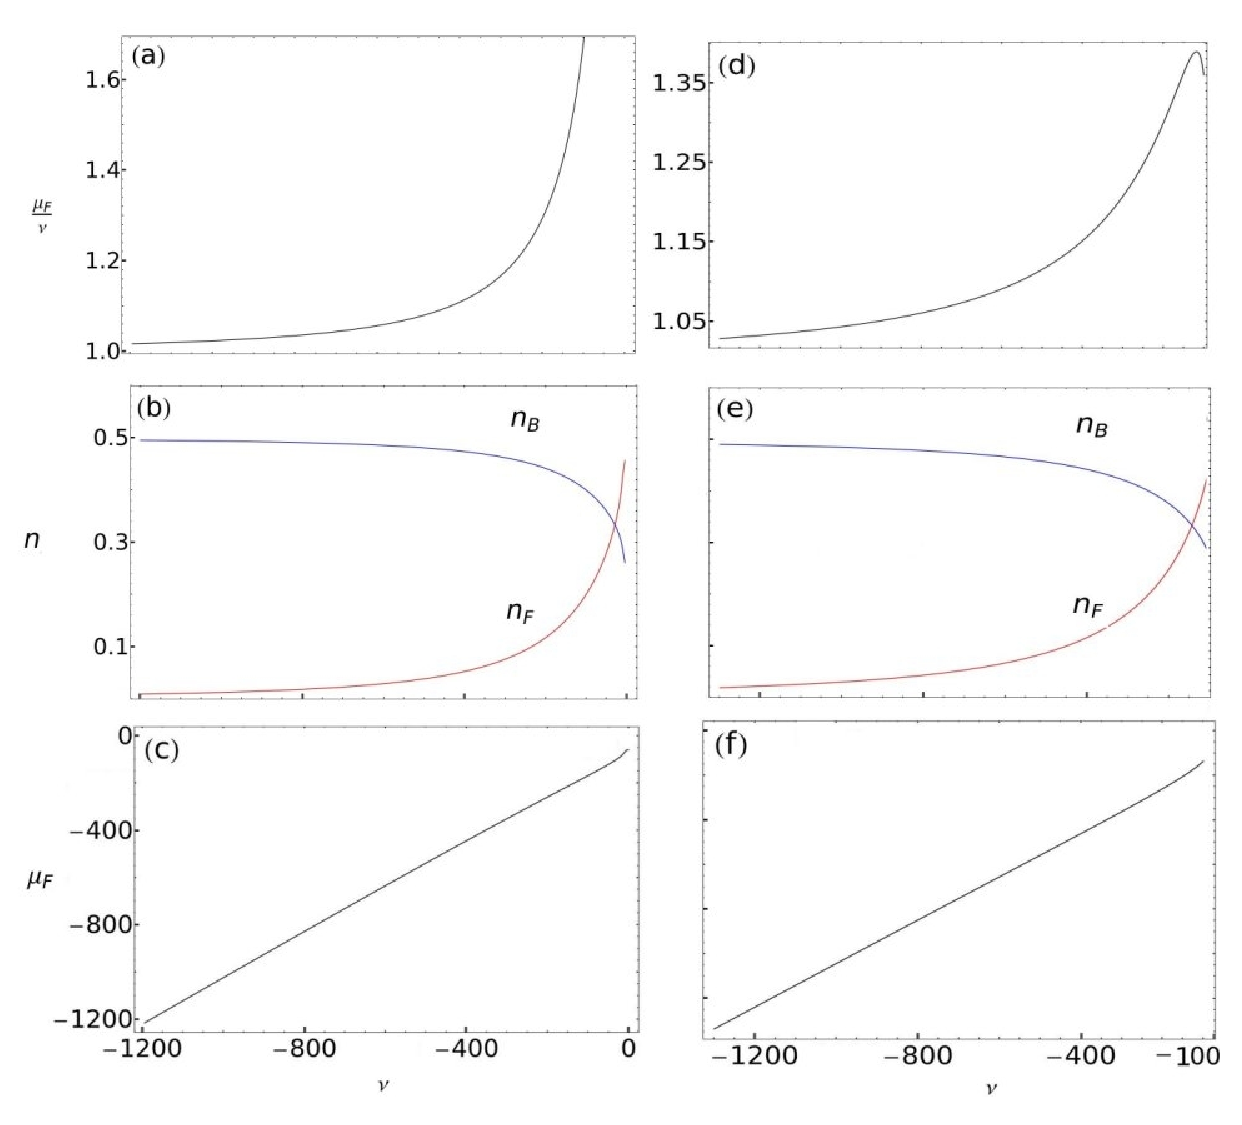
\epsfig{file=fig1.eps,height=5.6in,width=6in}
\caption{Plots of the  Fermion/Boson number and  chemical potential $\mu_F$  as a function of the Feshbach detuning $\nu$ in the deep-BEC and shallow-BEC regimes. Here, $\hbar = m =\mathcal{V} = 1$. Panels (a), (b) and (c) contain plots for the ratio $\mu_F/\nu$, the condensate fractions and $\mu_F$ respectively for $g_r=25$, $u_F = -0.3$, $u_B = 0$  and $\mathcal{N} = 100$. Panels (d), (e) and (f) contain plots for the ratio $\mu_F/\nu$, the condensate fractions and $\mu_F$ respectively for $g_r=40$, $u_F = -0.3$, $u_B = 0$  and $\mathcal{N} = 100$. In panels (b) and (e), the Fermion condensate fraction $n_F$ is shown in red, and the Boson molecular condensate fraction $n_B$  is shown in blue.}
\label{fig:chempot}
\end{figure}
Substituting this into the dynamics in eqns~\ref{dynamical_system}, dropping terms $\mathcal{O}(|\delta\Psi_j|^2)$ and higher, and separating the system into real and imaginary parts yields $\delta \dot{x}_j \sim \sum_k \mathcal{J}^{jk}_\nu\delta x_k$, where $\delta\Psi_{1,2}=\delta x_{1,3} + i \delta x_{2,4}$, and ${j,k}=1-4$. The Jacobian matrix elements that describe this dynamics are given by $\mathcal{J}^{jk}_\nu\equiv\partial\dot{x}_j/\partial x_k$.  
\begin{figure}[h!bt]
\begin{center}
\ 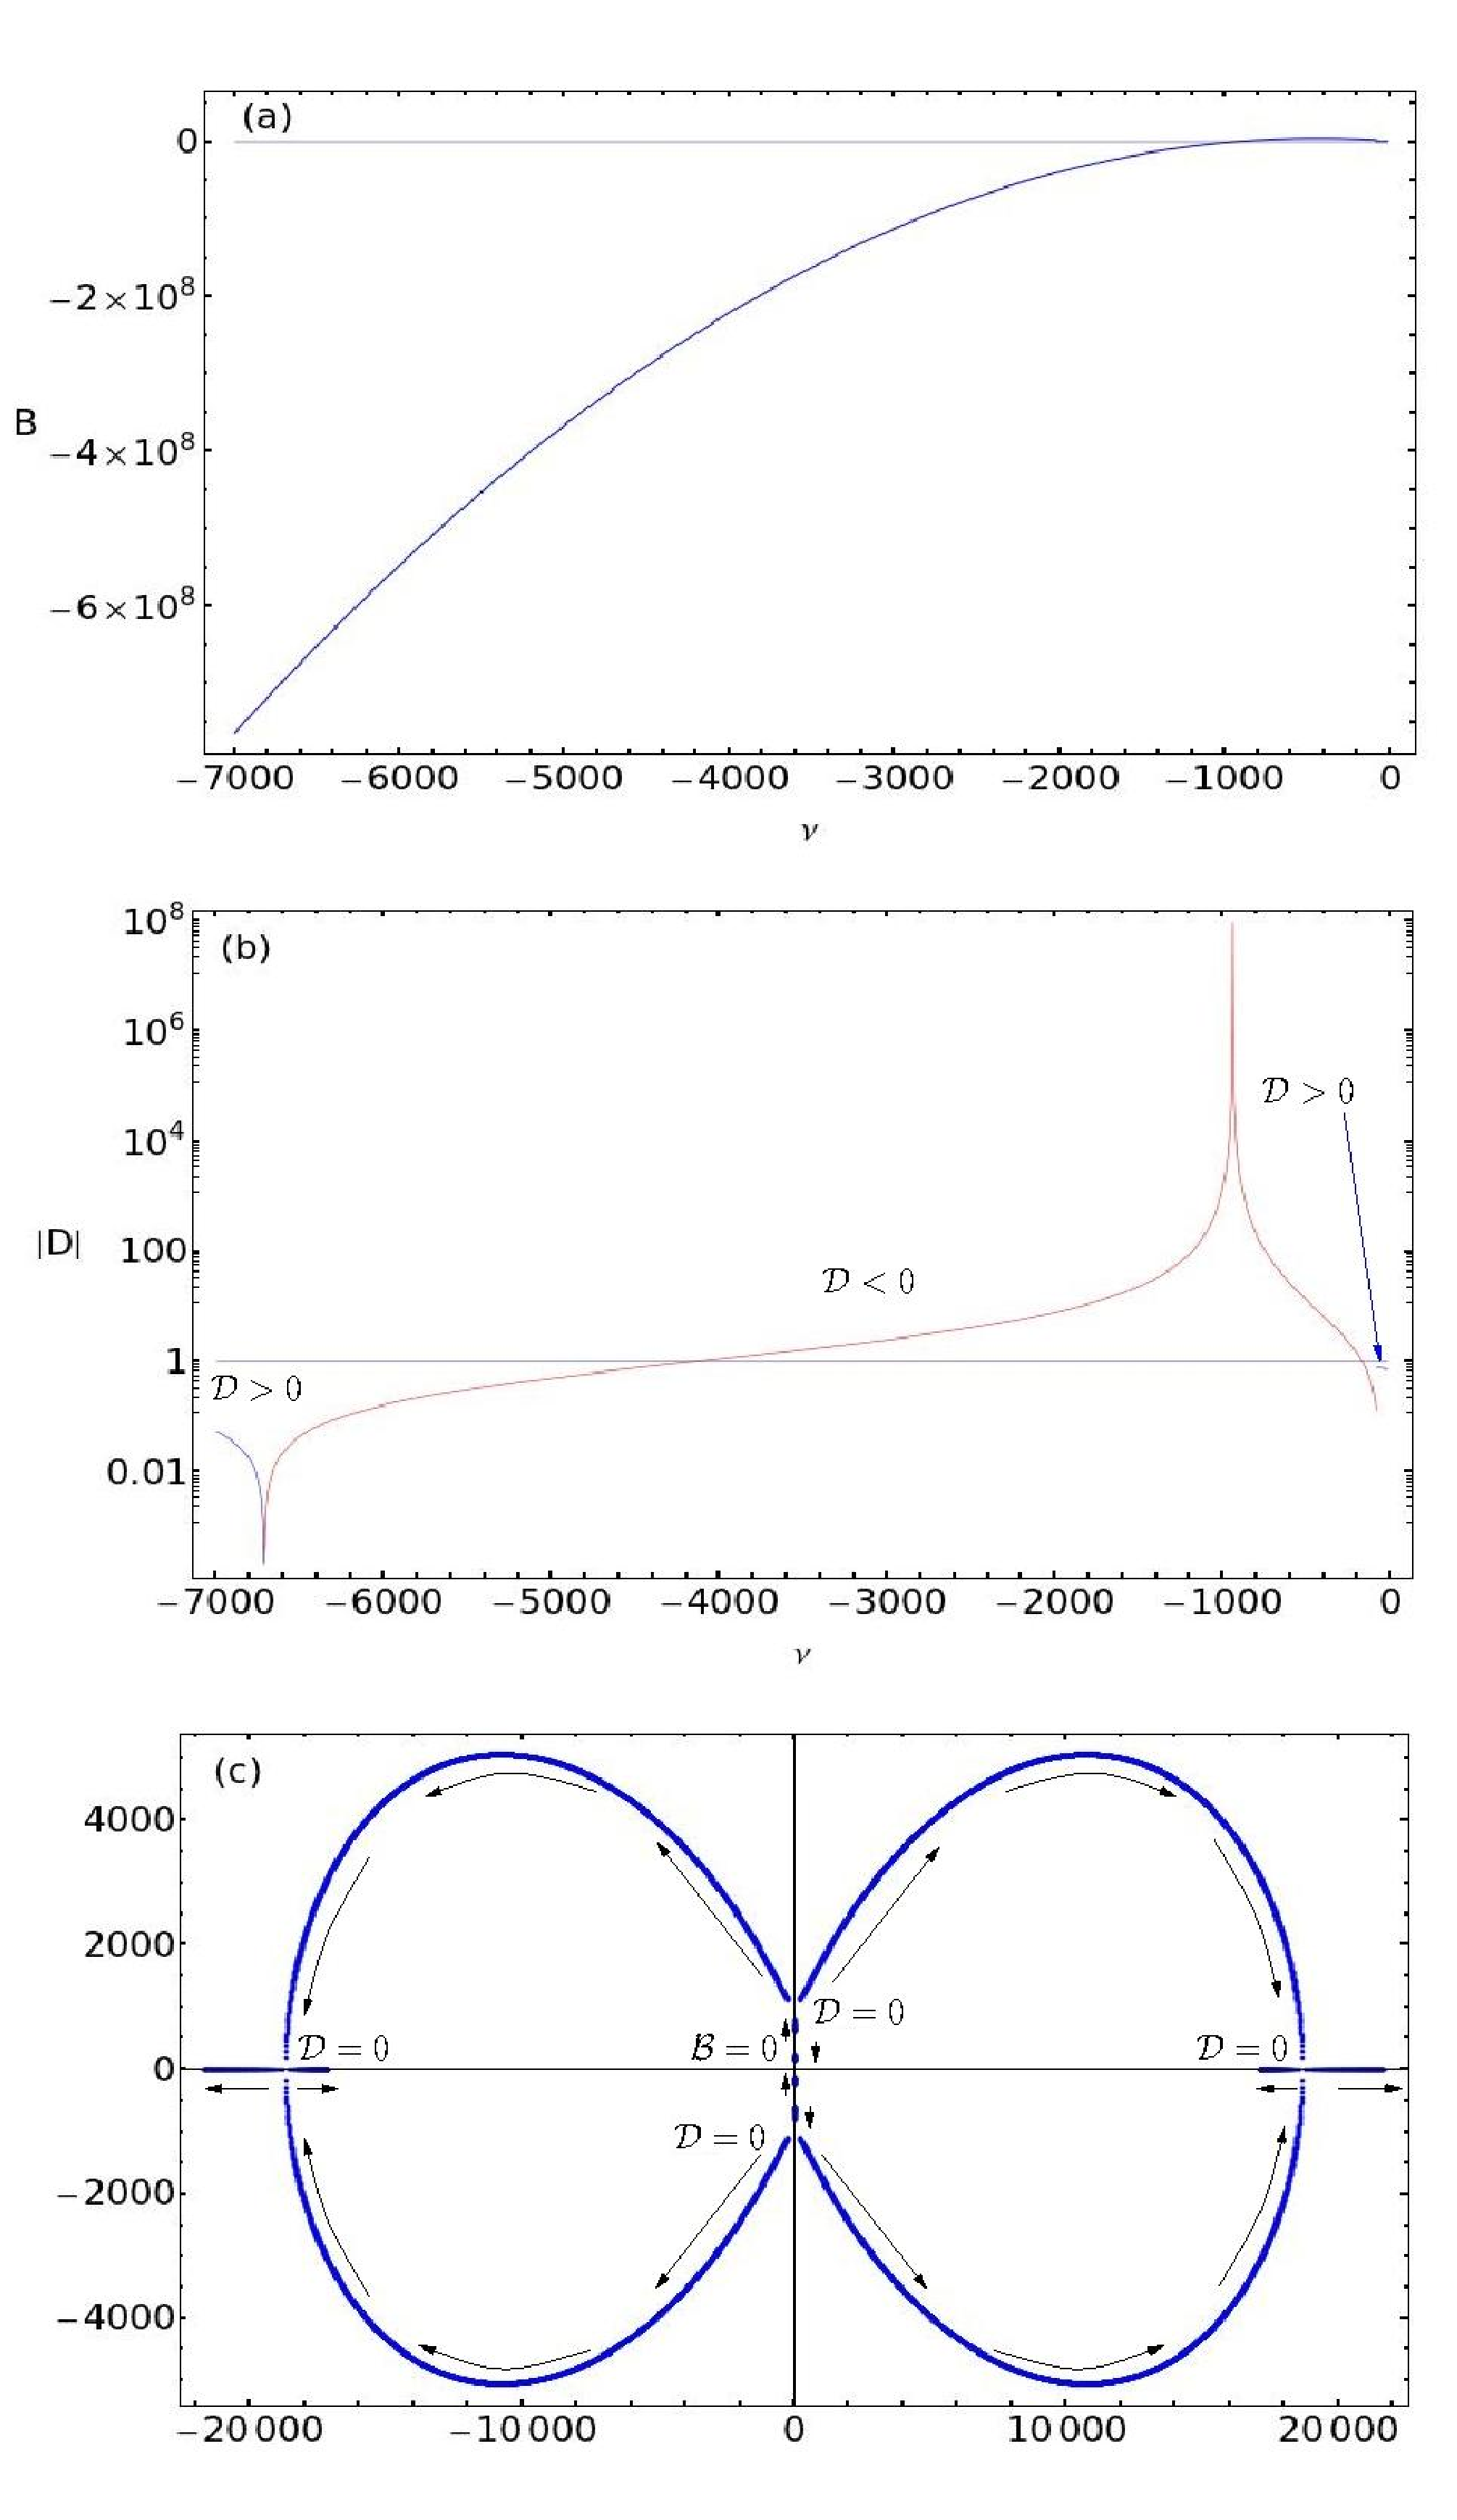
\epsfig{file=fig2.eps,height=5.6in,width=3.0in}
\end{center}
\caption{Bifurcation diagram in the complex plane of $\Omega_\nu$ obtained by numerically solving the BCS gap and number equations, applying the results to the Jacobian, and diagonalizing it. The numerics are performed for $100$ particles with $g_r=25$,$u_F = -0.3$,$u_B=0$, in a unit volume for unit particle mass, where $\hbar$ has also been set to unity. Panel (a) shows the coefficient $\mathcal{B}$ defined in eq~\ref{nobosonint:coeff} as a function of detuning $\nu$. Note that $\mathcal{B} > 0$ until $\nu \approx -943.77(0)$ and then switches sign. Figure (b) shows the magnitude of the discriminant $\mathcal{D}$ as a function of detuning $\nu$ in a semi-log plot. The regions of positive (negative) $\mathcal{D}$ are indicated in blue (red). Panel (c) shows the actual bifurcation diagram, with the roots $\Omega$ shown in the complex plane. The origin, where $\mathcal{B}=0$, is indicated, as well as the points where the 
discriminant $\mathcal{D}$ vanishes.}
\label{fig:bif:nobosonint}
\end{figure}
The eigenvalues $\Omega_\nu$ are given by the characteristic equation $|\mathcal{J}_\nu-\Omega_\nu I|=0$. In this case, the equation is biquadratic and yields $\Omega_\nu^4 + \mathcal{B}_\nu\Omega_\nu^2-\mathcal{C}_\nu =0$, where
\begin{eqnarray}
\label{roots:jacobian:nobosonint}
\Omega_\nu &=& \pm\sqrt{-\frac{\mathcal{B}_\nu}{2}}\left(1\pm\sqrt{\mathcal{D}_\nu}\right)^{1/2},\nonumber \\
 \mathcal{D}_\nu&\equiv& 1+\frac{4\mathcal{C}_\nu}{\mathcal{B}_\nu^2},\\
\label{nobosonint:coeff}
\mathcal{B}_\nu &\equiv& \beta r_\nu^2 \left[2\left(\alpha-\gamma\right)+3\beta r_\nu^2 \right]-\left(\alpha-\gamma\right)^2-
\frac{\left(\eta_\nu-3\right)\left(\eta_\nu+1\right)}{\left(\eta_\nu-1\right)^2}\times\kappa^2\gamma^2,\nonumber \\
\mathcal{C}_\nu &\equiv& \kappa^2\gamma^4+\frac{\left(\eta_\nu-3\right)\left(\eta_\nu+1\right)}{\left(\eta_\nu-1\right)^2}
\left[\left(\alpha-\gamma-2r^2_\nu\beta\right)^2-r^4_\nu\beta^2 \right]\kappa^2\gamma^2+2\kappa^2\gamma^3\left[\alpha-\gamma-\left(\frac{2\eta_\nu-1}{\eta_\nu-1}\right)r^2_\nu\beta\right].\nonumber \\
\end{eqnarray}
The quantity $\mathcal{D}_\nu$ is the \textit{discriminant} of the quartic equation. The linear dynamics is given by $|\delta x (t) \rangle \sim \sum^{4}_{j=1} c_j |\Omega^j_\nu\rangle e^{\Omega^j_\nu t}$, where $c_j$ are constants, $|\Omega^j_\nu\rangle$ are the eigenvectors of $\mathcal{J}_\nu$  that correspond to eigenvalues $\Omega^j_\nu$, and $|\delta x (t) \rangle$ is the vector given by $\delta x_{1-4}$. The sign of the quartic discriminant $\mathcal{D}_\nu$ plays a key role in determining the nature of these trajectories. If $\Omega_\nu$ are pure imaginary, the trajectories correspond to orbital motion about the radial fixed points.  When the $\Omega_\nu$ start to pick up real parts, then the trajectories corresponding to negative real parts are stable and decay in spirals to the orbits of the radial fixed points, thus creating a stable limit cycle. The eigenvalues with positive real parts are not expected to actually occur in these systems since they correspond to displacements that violate number 
conservation. Figure~\ref{fig:bif:nobosonint} (a) and (b) show plots of $\mathcal{B}_\nu$ and $\mathcal{D}_\nu$ as functions of detuning for the choice of parameters shown in the caption. Here, $\mathcal{B}_\nu$ is positive for small detuning and drops below zero at a critical value as $|\nu|$ is increased. Before that happens, however, $\mathcal{D}_\nu$ starts from a positive value that is less than unity. This means that the eigenvalues are pure imaginary. While $\mathcal{B}_\nu$ is still positive, the discriminant drops to negative values at $\nu\approx--88.6(0)$, and the roots  are now complex conjugate pairs. The value of $\mathcal{B}_\nu$ drops down to zero at around $\nu=-943.77(0)$, with the roots now vanishing at the origin. As $\mathcal{B}_\nu$ becomes negative, $\mathcal{D}_\nu$ is also negative and the roots retain their ongoing structure until $\mathcal{D}_\nu$ switches back to positive at around $\nu\approx-6715.(0)$, after which the roots are real with opposite signs. All these trends can be 
seen in the numerical evaluation of the eigenvalues plotted in the bifurcation diagram in figure~\ref{fig:bif:nobosonint} (c). Thus, a bifurcation is seen at the locus of $\mathcal{D}_\nu=0$ in the shallow-BEC regime. Here the limit cycles coalesce into orbital trajectories around the fixed points as the detuning $\nu$ is varied. 

Thus, the linear stability analysis of the fixed points demonstrates that the 'deep-BEC ' and 'shallow-BEC' regimes can be differentiated by the sign of the discriminant $\mathcal{D}_\nu$ inside these regimes. Finally, a rapid quench from the former to the latter can be expected to yield orbital phase space dynamics of $\Psi_j$ around the equilibrium fixed points after a sufficiently long time. Variations in the BEC number density, given by $|\Psi_2|^2 = x^2_3 + x^2_4$, is thus expected to show rapid nontrivial oscillations that can qualitatively resemble some sort of 'collapse and revival' of the matter wave packet. This can be seen in the numerical evaluation of eqs\ \ref{dynamical_system} for a sudden quench from the deep-BEC regime to the shallow BEC regime.The quenching is assumed to have taken place by a sharp variation of $\epsilon_F$ (via the Feshbach detuning $\nu$) from a large negative value (in the deep-BEC regime) to the shallow-BEC region. Figures~\ref{fig:colrev}(a)-(h) show the time variation 
of the BEC condensate fraction for the two representative parameter sets from figure~\ref{fig:chempot}  Figures~\ref{fig:colrev}(a) and (e) show the time evolution for very small times ($ \sim 10^{-2}$ units). In figures~\ref{fig:colrev}(b) and (f), discrete time samples of the actual signals are plotted in steps of $2\pi/\Omega_m$. The presence of another oscillation(s) of frequency $\Omega_e$ indicates that the actual signals contain a superposition of several comparably fast Rabi oscillations interfering with each other, and that $\Omega_e$ is their \textit{beat frequency}. For larger times, note from figures~\ref{fig:colrev}(c) and (g) that these beats damp out over a long period of time $t_d$, until a sudden onset of partial \textit{collapse and revival} of the matter wave begins after a short initial relaxation time $t_r$ (indicated in the respective figures). The \textit{revival time} $t_R$ is also indicated in the respective figures. The numerics plotted in fig~\ref{fig:colrev} indicate that the 
onset of this collapse and revival takes place at around $10^3$ numerical units. 

Plans to extend this work include a possible collaboration with Prof Avinash Khare of IISER, Pune, where we can investigate the stability of soliton trajectories in dynamical systems such as those of eqs.\ \ref{dynamical_system} with arbitrary nonlinearities and with gradient terms included. The stability of solitary waves in Gross-Piaevski systems of arbitrary nonlinearity (of the type $|\Psi|^k \Psi$ where the case discussed above encompasses $k=2$) in different dimensions is an ongoing discipline of study~\cite{khare}, and can be investigated using several techniques such as the Renormalization group~\cite{khare}, Derrick's Theorem and the Vakhitov and Kolokolov conjecture~\cite{derrick:vak}. The dimensionality plays a crucial role in the stability of such solutions and it should prove interesting to extend this formalism to coupled BCS-BEC systems as well. Other possibilities include the dynamics of fluctuations around the mean field, investigations in the deep-BCS regime at small temperatures, and 
quenches across the Breached Pair and FFLO state in population imbalanced Fermi Bose mixtures.

\begin{figure}[h!bt]
\ 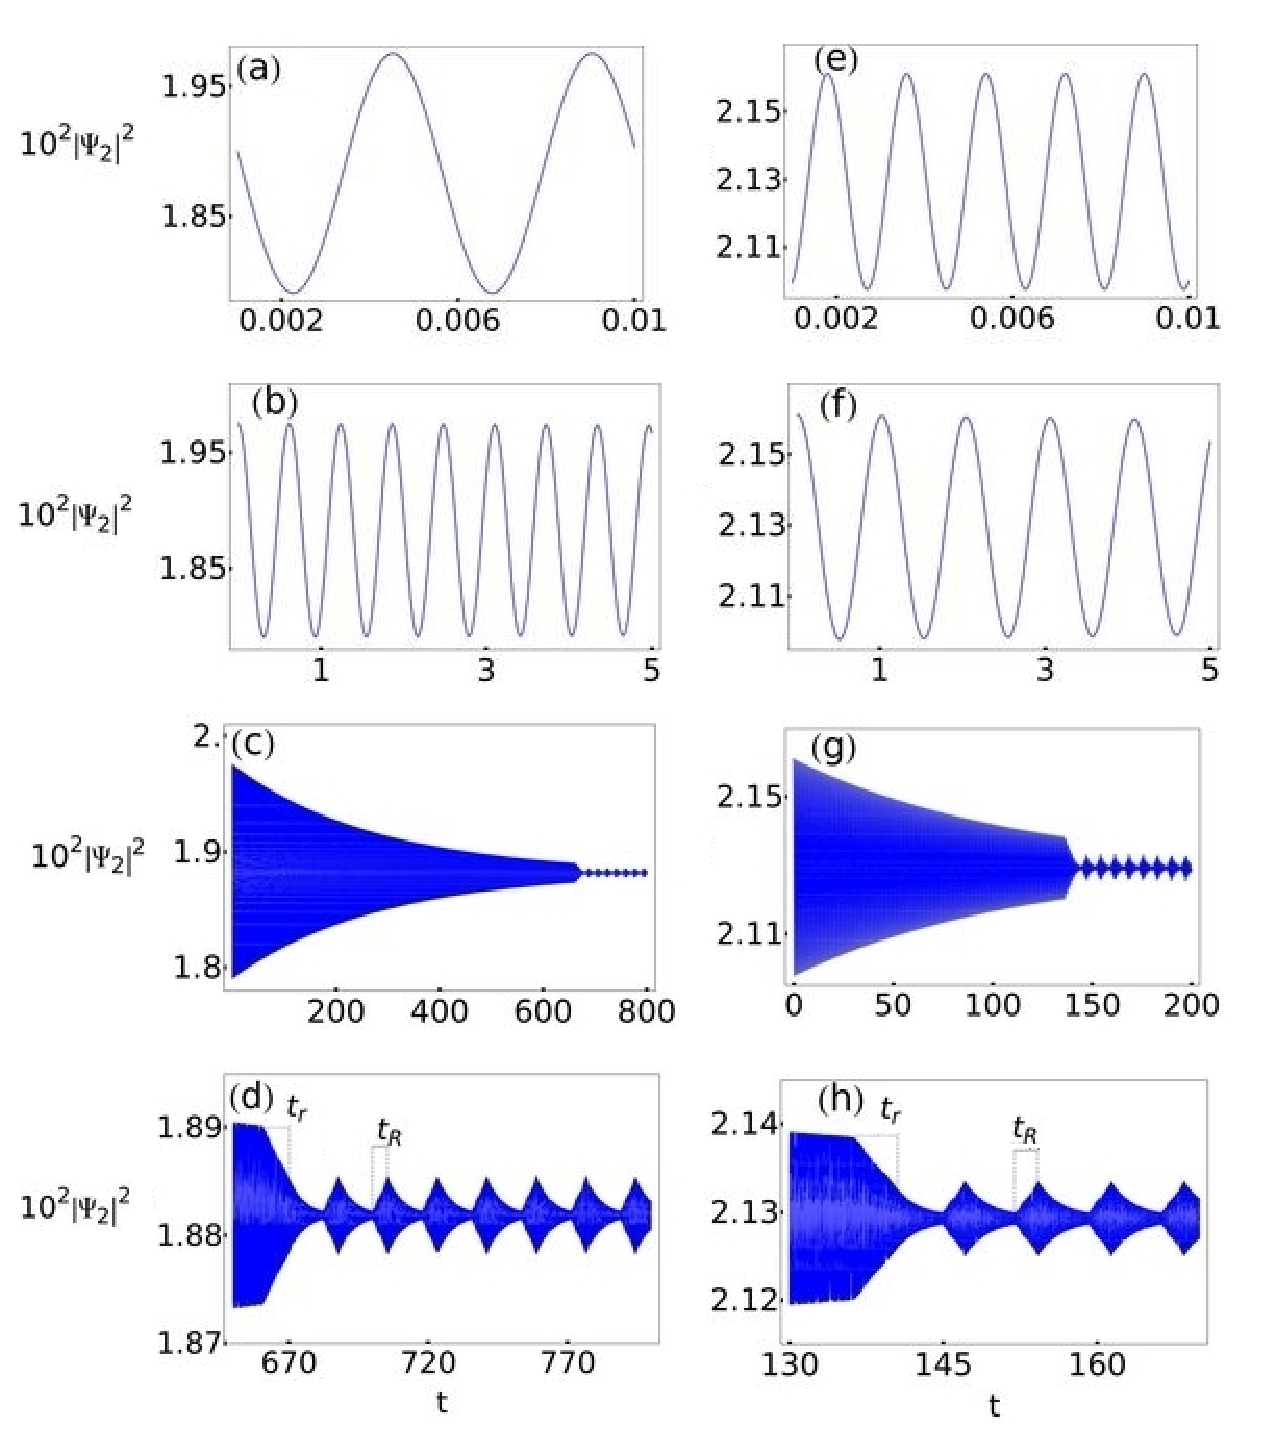
\epsfig{file=fig3.eps,height=5.6in,width=5.5in}
\caption{Plots of the signal $|\Psi_2|^2(t)$  from the solutions to equations~\ref{dynamical_system} for $u_B = 0$ after the system is quenched from a pure BEC to the shallow-BEC regime (see figure~\ref{fig:chempot}). Here, $\hbar = m =\mathcal{V} = 1$, and $u_F = -0.3$. Panels (a) - (d) show plots of the time evolution for $g_r=25.0$ and $\nu = -55.0$. Panels (e) - (h) show plots for $g_r=40.0$ and $\nu = -140.0$. Panels (a) and (e) show plots for very small times ($\sim 10^{-2}$). Panels (b),(c) and (f),(g) show plots of discrete time samples of the signal taken in units of the local time period from panels (a) and (e) respectively. Thus, panels (b),(c) and (f),(g) show the signals that envelope the master signal in (a) and (e) respectively. Panels (b),(c) and (f),(g) show the same corresponding envelope plots for two different time intervals. Partial collapse and revival of the matter wave can be seen after a lengthy decay time, where the original envelope damps out as it oscillates. The region where 
collapse and revival take place is magnified and shown in panels (d) and (h).}
\label{fig:colrev}
\end{figure}
\section{\sc Periodic dynamics of fermionic superfluids in the BCS regime}
\label{sec:fermidyn}

This section summarizes the research work concluded during the period beginning on January $1$, $2011$ and ending on August $31$, $2012$. The work is the result of a collaboration with Prof K. Sengupta and S. Modak (IACS, Kolkata), as well as Dr. Arnab Das (Max Planck, Dresden) and R. Dasgupta (SNBNCBS, Kolkata). The author is the primary contributor to this work and the principal author in the resultant publication(s). In this work, we study the non-equilibrium dynamics of a fermionic superfluid in the BCS limit and in the presence of a drive leading to a time dependent chemical potential $\mu(t)$. We choose a periodic driving protocol characterized by a frequency $\omega$ and compute the fermion density, the wavefunction overlap, and the residual energy of the system at the end of $n$ periods of the drive. We demonstrate that the BCS self-consistency condition is crucial in shaping the long-time behavior of the fermions subjected to the drive and provide an analytical understanding of the behavior of the 
fermion density $n_{k_F}$ (where $k_F$ is the Fermi momentum) after a drive period and for large $\omega$. This work has been uploaded to arXiv, and has been sent to Physical Review A for peer review~\cite{mypaper2}.

The Hamiltonian for a gas of interacting ultracold fermions in a shallow square optical lattice, in
the absence of any drive, is given by
\begin{equation}
H(t) = \sum_{{\bf k}\sigma} \left[ \epsilon_{\bf
k}-\mu_0\right]c^\dagger_{{\bf k}\sigma}c_{{\bf k}\sigma} -g \sum_{{\bf k}, {\bf k'},{\bf k''}} c^\dagger_{{\bf k}+{\bf
k''}\uparrow} c^\dagger_{{\bf k'}-{\bf k''}\downarrow} c_{{\bf
k'}\downarrow} c_{{\bf k}\uparrow}. \label{fermiham}
\end{equation}
Here $c_{{\bf k}\sigma}$ represent the annihilation operators for fermions of momentum ${\bf k}$ and spin $\sigma=\{\uparrow,
\downarrow\}$. The first term represents the kinetic energy of the fermions, and the second term the four-fermion interaction energy
with amplitude $g>0$ which represents attractive interaction between the fermions. Here $\epsilon_{\bf k}= -2J \sum_{i}\cos(k_i)$ is the
band energy spectrum for the fermions, the index $i$ takes values $x$ and $y$ for $d=2$ or $x$, $y$, and $z$ for $d=3$, and $\mu_0$ is
the chemical potential. In the BCS regime and at zero temperature,
the ground state of the fermions is a superfluid whose excitations
can be described by the BdG equations
\begin{eqnarray}
E({\bf k})\left(\begin{array}{c} u_{\bf k} \\ v_{\bf k}
\end{array} \right) &=& \left(
\begin{array}{cc}
(\epsilon_{\bf k}-\mu_0) & \Delta({\bf k})\\
\Delta^{\ast}({\bf k}) & -(\epsilon_{\bf k}-\mu_0)
\end{array} \right) \left(\begin{array}{c} u_{\bf k} \\ v_{\bf k}
\end{array} \right), \nonumber\\ \label{bdg1}
\end{eqnarray}
where $u_{\bf k}$ and $v_{\bf k}$ are the amplitudes of the particle
and the hole in a BdG quasiparticle and are related to the BCS
wavefunction by
\begin{eqnarray}
|\psi\rangle &=& \prod_{\bf k} (u_{\bf k} + v_{\bf k} c_{\bf
k}^{\dagger} c_{{\bf -k}}^{\dagger}) |0\rangle. \label{bcswav}
\end{eqnarray}
The pair-potential $\Delta({\bf k})$ depends on the pairing symmetry
and is given by
\begin{eqnarray}
\Delta({\bf k}) &=& \Delta_0, \quad {\rm s-wave }, \nonumber\\
\Delta({\bf k}) &=& \Delta_0 [\cos(k_x) -\cos(k_y)],  \quad {\rm
d}_{x^2-y^2}{\rm -wave}. \label{pp}
\end{eqnarray}
For s-wave pairing, the pair potential satisfies the
self-consistency relation
\begin{eqnarray}
\Delta_0 &=& g \sum_{\bf k} u_{\bf k}^{\ast} v_{\bf k}.
\label{self1}
\end{eqnarray}
Eq.\ \ref{bdg1} and \ref{self1} admit the well-known BCS solution
\begin{eqnarray}
E({\bf k})&=& \pm \sqrt{(\epsilon_{{\bf k}}-\mu_0)^2+|\Delta_0|^2}
\nonumber\\
u^{\rm eq}_{\bf k} (v^{\rm eq}_{\bf k}) &=& \frac{1}{{\sqrt 2}}
\left( 1+(-) \frac{(\epsilon_{\bf k} -\mu_0)}{E({\bf k})}
\right)^{1/2}. \label{eqsol}
\end{eqnarray}
We now introduce a time-dependent drive, $\mu(t)=\mu_0 +\mu_a
\sin(\omega t)$, so that $\mu_a, \,  \omega \ll J $. This can be
achieved in typical experimental systems by introducing an
additional time-dependent harmonic trap potential which is
sufficiently broad so as to allow for a uniform fermion density. In
this regime, the response of the system to the drive can be
described by the time-dependent Bogoliubov de-Gennes equation given
by
\begin{equation}
i \partial_t \left(\begin{array}{c} u_{\bf k}(t) \\ v_{\bf k}(t)
\end{array} \right) = \left(
\begin{array}{cc}
(\epsilon_{\bf k}-\mu (t)) & \Delta({\bf k;t})\\
\Delta^{\ast}({\bf k};t) & -(\epsilon_{\bf k}-\mu (t))
\end{array} \right) 
\times \left(\begin{array}{c} u_{\bf k}(t)\\ v_{\bf k}(t)
\end{array} \right), \label{bdg2}
\end{equation}
together with the self-consistency condition which, for s-wave
pairing, reads
\begin{eqnarray}
\Delta({\bf k};t) &\equiv& \Delta(t) = g \sum_{\bf k} u^{\ast}_{\bf
k}(t) v_{\bf k}(t).\label{tdsc1}
\end{eqnarray}
\begin{figure}
\begin{center}
\rotatebox{0}{\includegraphics*[width=5in]{fig4.eps}}
\end{center}
\caption{  Plots of the long time average and
instantaneous values of the amplitude of the order parameter
$\Delta(t)$. The left panel shows the plot of the long time averaged
$|\Delta(t)|$ (averaged over $10$ cycles of the drive) with respect
to the drive frequency $\omega$. The right panel shows variation of
the instantaneous values of $|\Delta(t)|$ with time $t$ (in units of
$2\pi/\omega$) for several representative values of $\omega$
indicated in the legend. In both panels, $\Delta_0$ is indicated by
a black dashed horizontal line.} \label{fig4}
\end{figure}
In the rest of this work, we consider the system to be in the
superfluid ground state at $t=t_i$ with $(u_{\bf k}(t_i), v_{\bf
k}(t_i)) =(u^{\rm eq}_{\bf k}, v_{\bf k}^{\rm eq})$ and study its
evolution in the presence of the periodic drive till a time $t_f$
which correspond to $n$ cycles of the drive $t_f =nT=2\pi n/\omega$,
where $n$ is an integer.

In order to study such dynamics, we focus on the effective magnetization $m(t)$
defined as
\begin{eqnarray}
m_{\bf k}(t) &=& \langle \psi_{\bf k}(t)| \tau_z |\psi_{\bf k}(t)\rangle, \nonumber \\
m(t) &=& \sum_{\bf k} m_{\bf k}(t) = \sum_{\bf k} [1-2|v_{\bf
k}(t)|^2 ],\label{eq:mag}
\end{eqnarray}
where $\tau_z$ is the Pauli matrix in particle-hole space. The
observable $m(t)$ shall be equal to $m(t_i)$ after a full drive
cycle at $T=2\pi/\omega$ both in the impulse (where the wavefunction
does not have time to adjust to the drive) and adiabatic limit
(where the system remains in the ground state of the instantaneous
Hamiltonian). Note that $m(t)$ is the magnetization of the Ising or
Kitaev models described by BdG-like equations in their fermionic
representations sans the self-consistency
condition\cite{arnab1,diptiman}. If the time dependence of $\Delta$ is ignored or rendered
negligible, then the system reverts to an ensemble of decoupled
two-level systems in momentum space with constant gap $\Delta_0$. In
this case, the dynamics is described by Landau-Zener-St\"uckelberg
theory~\cite{review:lzstls}. As we shall see in the next paragraph, we
reach this regime for $ \omega/\Delta_0 \ll 1$; however, the
behavior of a BCS system differs significantly from that of a bunch
of decoupled two-level system for moderate $\omega$ for which
$\omega/\Delta_0 \sim 1$.

Now, we discuss the self-consistent numerical evaluation of Eqs.\ \ref{bdg2} and \ref{tdsc1} for $d=2$ and subsequent
computations of $m(t)$, and $|\Delta(t)|$, as
defined above. We have solved Eq.\ \ref{bdg2} and
\ref{tdsc1} for BCS fermions in a $144\times144$ square optical
lattice and having  unit hopping amplitude ($J=1$). The equilibrium
gap and chemical potential has been taken to be $\Delta_0=0.1$ and
$\mu_0=0.01$ respectively. The periodic drive term has been taken to
be of the form $\mu_a \sin(\omega t)$ with $\mu_a=0.1$.

We first consider the plot of the gap amplitude $|\Delta|$ in Fig.\
\ref{fig4}. The left panel of Fig.\ \ref{fig4} shows the average gap
amplitude as a function of the drive frequency $\omega$ after an
average over $10$ cycles. We find that the average value of the gap
amplitude decreases rapidly with increasing frequency and keeps
fluctuating about $|\Delta| \simeq 0.2 \Delta_0$ for large
$\omega/\Delta_0 \ge 2$. The right panel shows a plot of
$|\Delta(t)|/\Delta_0$ as a function of $\omega t/2\pi$. We find
that at small $\omega \ll \Delta_0$, $|\Delta(t)|$ displays
oscillatory behavior with maximum and minimal values of $\Delta_0$
and $0.9 \Delta_0$ respectively. However, for $\omega \ge \Delta_0$,
the behavior of $|\Delta(t)|$ is qualitatively different; it
decreases rapidly to near-zero values within the first couple of
drive cycles ($\omega t/2\pi \le 2$) and continues to fluctuate
around this value for longer drive times, never returning close to
its original value $\Delta(0)$. We note that such a behavior of
$|\Delta(t)|$ clearly reflects the importance of the
self-consistency condition in the dynamics; any analysis with
$|\Delta(t)| \simeq \Delta_0$ at all times is expected to produce
qualitatively wrong results for $\omega \ge \Delta_0$.

Next, we plot the effective magnetization $m(t)$ as a function of
time $t$ and its time average $Q$ as a function of the drive
frequency $\omega$. For the {\it self-consistent} dynamics
appropriate for fermions in the BCS regime, as shown in Fig.\
\ref{fig5}, there are clearly three regimes, one crossing over to
the other as $\omega$ is increased. For $\omega \ll \Delta_{0}$,
$m(t)$ (right panel) oscillates with large amplitude, following the
drive almost adiabatically, resulting in $Q = m(0)$. The
oscillations, though large, respects the symmetry of the drive. As
$\omega$ approaches $\Delta_{0}$, this symmetry is destroyed,
resulting $Q \ne m(0)$. For $\omega > \Delta_{0}$, the oscillatory
behavior of $m(t)$ with large amplitude is replaced by relaxation to
an approximately constant value (with negligible fluctuations)
within few initial cycles (right panel). This constant value
determines the value of $Q$ (left panel), and we find that it
deviates steadily from $m_{0}$ as $\omega$ is increased for $\omega
< 2.5 \Delta_0$. We note that for $\omega > \Delta_0$, the mixing of
the ${\bf k}$ modes of the quasiparticle excitations, which
originates from the presence of the self-consistency condition and
is therefore absent in Ising or Kitaev systems, is at the heart of
such a deviation. The freezing of magnetization breaking the
symmetry of the driving, seen here for $\omega \le \Delta_0$, was
observed in Ref.\ \cite{arnab1} for periodically driven
transverse Ising chain for large amplitude and frequency. For very
large $\omega$, we of course see the behavior of $m(t)$ crossing
over to a regime where $Q \rightarrow m(0)$ again -- here $\omega$
becomes too large for the system to react at all, and $m(t)$ remains
frozen around $m(0)$ for all time (the regime sets in beyond $\omega
> 2.4$).

The above behavior is to be contrasted with the {\it
non-self-consistent} case summarized in Fig.\ \ref{fig6}. Here
$m(t)$ always executes a large, almost synchronized oscillation,
approximately following the adiabatic path (black crosses in the
right panel of Fig.\ \ref{fig6}). Naturally, the resulting values of
$Q$ are close to $m(0)$ (albeit with some small fluctuations). This
suggests that the synchronous oscillation is simply a manifestation
of the near-adiabatic nature of the dynamics. Synchronization could
also occur due to self dephasing of the system, after all the
transients (some of them having power-law tails) have died down, due
to quantum interference between the modes \cite{arnab1}.
But such synchronization would appear only in the $\omega t
\rightarrow \infty$ limit, unlike in the present case, where the
effect is visible from the very first cycle. The qualitative
departure from this behavior in the self-consistent case seems to
stem form the non-adiabaticity induced by the self-consistency
condition (Eq.\ \ref{tdsc1}) which makes the effective Hamiltonian
non-linear. The overlapping eigenfunctions of the non-linear
Hamiltonian makes the criteria for adiabatic behavior much more
restricted compared to a linear case. We shall address the behavior of $m_{k_F}(t)$
in a more quantitative manner below, where we
shall show that the value of $m_{k_F}$ after one drive cycle decays
as $1/\omega$ for $\omega \gg \Delta_0$.

Finally, we obtain an analytical understanding of the
behavior of the magnetization or fermion density at the gap edge,
{\it i.e.} at $|{\bf k}|= k_F$, after a drive cycle in the
high-frequency limit. We derive a picture analogous to that of 
\begin{figure}
\begin{center}
\rotatebox{0}{\includegraphics*[width=5in]{fig5.eps}}
\end{center}
\caption{  Left Panel: Plot of $Q$ as a function of
$\omega$ with averaging carried over $10$ drive cycles. Right panel:
Plot of $m(t)$ as a function of $\omega t/2\pi$ for representative
values of $\omega$ indicated in the legend. A few representative
values of the adiabatic magnetization $m^{adb}(t)$ is shown using
crosses. In both panels, the initial values of $Q$ and $m$ is
indicated by a magenta dashed horizontal line and all parameters are
same as in Fig.\ \ref{fig4}} \label{fig5}
\begin{center}
\rotatebox{0}{\includegraphics*[width=5in]{fig6.eps}}
\end{center}
\caption{  Same as in Fig.\ \ref{fig5} but for the
non-self-consistent dynamics.} \label{fig6}
\end{figure}
the non self-consistent dynamics for a two-level
system described above, except {\it with the self-consistency condition} updating the dynamics at all times. The calculation
is carried out here for s-wave superfluids but can be easily
generalized to other pairing symmetries. Defining the terms
\begin{eqnarray}
\label{eq:akbk}
s_{\bf k}(t) &=& \exp\left\{-i\int^t_0\mathrm{d}t' {\left[\epsilon_{\bf k}-\mu(t') \right]}\right\},\nonumber \\
u_{\bf k}(t) &=& a_{\bf k}(t) s_{\bf k}(t),\quad v_{\bf k}(t) =
b_{\bf k}(t) s^{-1}_{\bf k}(t),
\end{eqnarray}
the dynamics of the system in eqs.\ \ref{bdg2} and\ \ref{tdsc1} can be rewritten as
\begin{eqnarray}
\label{eq:akbkdyn0}
\dot{a}_{\bf k} &=& -i\Delta(t)b_{\bf k}(t) s^{-2}_{\bf k}(t),\nonumber \\
\dot{b}_{\bf k} &=& -i\Delta^\ast(t)a_{\bf k}(t) s^{2}_{\bf k}(t), \nonumber  \\
\Delta(t) &=& g \times \exp{\left[i\int^t_0{\mathrm d}t'\mu'(t')\right]} \sum_{\bf k}a^\ast_{\bf k}(t)b_{\bf k}(t)
e^{2if_{\bf k}t},
\end{eqnarray}
where $f_{\bf k}= \epsilon_{\bf k}-\mu_0$ and
$\mu'(t)=\mu_a\sin{\omega t}$. The initial conditions for $a_{\bf
k}$ and $b_{\bf k}$ can be easily obtained from those of $u_{\bf k}$
and $v_{\bf k}$. We note that the adiabatic dynamics has an avoided crossing at $t_{1{\bf
k}} = t_1 = \arcsin(f_{\bf k}/\mu_a)/\omega$ and that $t_1$
approaches zero for large $\omega$ and for all momenta on the Fermi
surface. Further if $\omega t_1 \ll 1$, a condition which is exactly
satisfied at $|{\bf k}|=k_F$, we may use the Zener approximation
$\mu'(t)\approx\mu_a\omega t$ for $\mu(t)$ close to $t=t_1$ when the
system traverses the avoided
crossing~\cite{review:lzstls},
and restrict ourselves within the adiabatic impulse model where all
excitations away from the avoided crossing are
ignored~\cite{review:lzstls}. From the definitions in Eq.\
\ref{eq:akbk}, we can simplify Eq.\
\ref{eq:akbkdyn0} to yield
\begin{equation}
\label{eq:akdyn} \dot{a}_{\bf k} = -i\Delta(t) b_{\bf k}(t)
e^{2i\left(f_{\bf k}t-\frac{1}{2}\mu_a\omega t^2\right)}.
\end{equation}
This equation can be integrated~\cite{mypaper2} to yield the amplitude $a_{\bf k}(t)$ after traversing one avoided crossing
\begin{equation}
\label{eq:afkfinal} \mathcal{A}^{(1)}_{\bf k} = u^{\rm eq}_{\bf
k}- \sqrt{\frac{\pi\Delta^2_0}{\mu_a\omega}}
e^{i\left(\frac{f^2_{\bf
k}}{\mu_a\omega}+\frac{\pi}{4}\right)}  \times \sum^\infty_{n=0} \frac{1}{n!}
\frac{\left(-i\right)^n}{\left(4\mu_a\omega\right)^n}
\frac{\partial^{2n}\theta_{\bf k}}{\partial^{2n}t}\bigg|_{t=t_{\bf
k}},
\end{equation}
\begin{figure}
\begin{center}
\rotatebox{0}{\includegraphics*[width=3in]{fig7.eps}}
\end{center}
\caption{Numerical plots (blue crosses) of $m_{k_F}$
as a function of $\omega$. The system parameters are the same as in
Fig.\ \ref{fig4}. The red solid line indicates the analytical result
obtained in Eq.\ \ref{meqfinal}.} \label{fig:magcomp}
\end{figure}
where $\theta_{\bf k}(t) =  b_{\bf k}(t) \Delta(t)/\Delta_0=v_{\bf
k}(t)s_{\bf k}(t)\Delta(t)/\Delta_0$, and $\mathcal{A}^{(n)}_{\bf k}$ denotes the amplitude $a_{\bf k}$
after $n$ passages across the avoided crossings with
$\mathcal{A}^{(0)}_{\bf k}$ being the initial amplitude of $a_{\bf
k}$, and we have used $a_{\bf k}(0)=u^{\rm eq}_{\bf k}$ from Eq. \
\ref{eq:akbk}, and $t_{\bf k}= f_{\bf k}/(\mu_a \omega)$. Restricting ourselves to a small region around the Fermi surface (given by $f_{\bf k}=0$), we obtain the fermion density after one passage
\begin{eqnarray}
\label{eq:lzmod}
|\mathcal{B}^{(1)}_{\bf k}|^2 &=& 1 - |\mathcal{A}^{(1)}_{\bf k}|^2 \nonumber \\
    &=& 1-\Big[\left(u^{\rm eq}_{\bf k}\right)^2+\chi_0|c_{\bf k}|^2 - 2u^{\rm eq}_{\bf k}\sqrt{\chi_0}\times{\rm Re}\left(c_{\bf
k}e^{i\kappa_{\bf k}}\right)\Big],
\end{eqnarray}
where we have defined
\begin{eqnarray}
\label{eq:ckchieta} c_{\bf k} &=& \sum^\infty_{n=0} \frac{1}{n!}
\frac{\left(-i\right)^n} {\left(4\mu_a\omega\right)^n}
\frac{\partial^{2n}\theta_{\bf
k}} {\partial^{2n}t}\bigg|_{t=t_{\bf k}}, \nonumber\\
\kappa_{\bf k} &=& \frac{f^2_{\bf k}}{\mu_a\omega}+\frac{\pi}{4},
\quad \chi_0 = \frac{\pi\Delta^2_0}{\mu_a\omega}.
\end{eqnarray}
{Noting that for $\omega \gg f_{\bf k}$, $\kappa_{\bf k} \sim
\pi/4$, and approximating}
\begin{equation}
\label{eq:ck0} c_{\bf k} \approx \sum^\infty_{n=0} \frac{1}{n!}
\frac{\left(-i\right)^n}{\left(4\mu_a\omega\right)^n}
\frac{\partial^{2n}\theta_{\bf k}}{\partial^{2n}t}\bigg|_{t=0},
\end{equation}
one finally gets an expression for the modified Landau-Zener
probability
\begin{eqnarray}
\label{eq:lz:pert} |\mathcal{B}^{(1)}_{\bf k}|^2 &=& \left(v^{\rm
eq}_{\bf k}\right)^2 -\chi_0|c_{\bf k}|^2+u^{\rm eq}_{\bf
k}\sqrt{2\chi_0}{\rm Re}\left[\left(1+i\right)c_{\bf k}\right]
\nonumber\\
\end{eqnarray}
Each of the terms in the sum of Eq.\ \ref{eq:ck0},and higher order derivatives thereof, can be obtained
from the initial conditions in eq\ \ref{eqsol}, together with the dynamics in eqs\ \ref{bdg2} and \ref{tdsc1}. Close to the Fermi surface,
eq\ \ref{eq:ckchieta} can be simplified and approximated by retaining terms up to order $n=1$ to yield an approximation for the fermion density after one passage
\begin{equation}
\label{eq:b1} |\mathcal{B}^{(1)}_{\bf k}|^2  \approx |v^{\rm
eq}_{\bf k}|^2\left[1+\frac{\chi^{1/2}_0}{\sqrt{2}}\frac{u^{\rm
eq}_{\bf k}}{v^{\rm eq}_{\bf k}}\right],
\end{equation}
where only the lowest contributing order of $\chi_0$ is retained. After one complete period
\textit{i.e} two passages across the avoided crossing, the fermion
density in the adiabatic impulse limit is given
by~\cite{review:lzstls}
\begin{eqnarray}
\label{eq:prob:1p}
 |\mathcal{B}^{(2)}_{\bf k}|^2 &=& 2 |\mathcal{B}^{(1)}_{\bf k}|^2
 \left(1-|\mathcal{B}^{(1)}_{\bf k}|^2\right)\nonumber \\
 &=&2\bigg[\left(u^{\rm eq}_{\bf k}v^{\rm eq}_{\bf k}\right)^2\left(1-\frac{\chi_0}{2}\right) +u^{\rm eq}_{\bf k}v^{\rm eq}_{\bf k}\left(|u^{\rm eq}_{\bf k}|^2-|v^{\rm eq}_{\bf k}|^2\right)\sqrt{\frac{\chi_0}{2}}\bigg],
\end{eqnarray}
Thus the magnetization $m_{\bf k}^{(2)}$ after
one period (or two passages across the avoided crossing) can be
evaluated using Eqs.\ \ref{eq:mag} and\ \ref{eq:prob:1p}, yielding
\begin{eqnarray}
\label{eq:m2:ex} m^{(2)}_{\bf k} &\simeq&
1-4\left(1-\frac{\chi_0}{2}\right) \left(u^{\rm eq}_{\bf k}v^{\rm
eq}_{\bf k}\right)^2 +\sqrt{8\chi_0} u^{\rm eq}_{\bf k}v^{\rm
eq}_{\bf k}m^{\rm eq}_{\bf k}, \nonumber\\
\end{eqnarray}
where $m^{\rm eq}_{\bf k}$, the equilibrium magnetization, is given
by $m^{\rm eq}_{\bf k}=1-2|v^{\rm eq}_{\bf k}|^2$. Thus at $|{\bf
k}|=k_F$, where all approximations used to arrive at this result are
clearly valid, one obtains, using $u_{k_F}^{\rm eq} = v_{k_F}^{\rm
eq}=1/\sqrt{2}$,
\begin{eqnarray}
m^{(2)}_{k_F} \equiv m_{k_F} = m_0 \frac{\Delta_0}{\omega}, \quad
m_0 = \frac{\pi \Delta_0}{2 \mu_a}. \label{meqfinal}
\end{eqnarray}
Thus, we find that the frequency dependence of the magnetization (or
equivalently the fermion density) is $m_{k_F} \sim\omega^{-1}$. The
magnetization drops off at the same manner as the non
self-consistent case (\textit{i.e} the driven Ising model where
$m\sim\omega^{-1}$ can be obtained from the Landau Zener formula).
The constant $m_0$ which decides the rate of the decrease of
$m_{k_F}$ with $\omega$, however, is different in the two cases. The generalization of this treatment to $n$ periods
seems to be difficult due to the necessity of taking into account
multiple Stuckelberg phases and we leave this issue for a possible
future study. This analytical result is compared with numerical results for the magnetization on the
Fermi surface after one drive period in fig.\ \ref{fig:magcomp}. The agreement is quite good for $\omega \ge 3
\Delta_0$ but poor for smaller $\omega/\Delta_0$ where some of the
approximations made in this treatment are clearly violated.
 
In conclusion, we have studied the non-equilibrium periodic dynamics of Fermi superfluids in the BCS regime
within a self-consistent mean-field theory. We have shown that proper incorporation of the self-consistency
condition is crucial for understanding the dynamic properties of such systems. This is particularly highlighted by
studying the behavior of the effective magnetization $m(t)$ which shows qualitatively different
behavior for Fermi superfluids (which obey self-consistent BCS equations) and Ising or Kitaev spin models (whose properties are governed by BCS-like equations without the self-consistency condition). Finally, we have provided an analytical derivation of the frequency dependence of the magnetization at the end
of one drive cycle in the limit of large drive frequency and have shown that it scales as $\omega^{-1}$ for large $\omega$. 

We are currently extending this formalism to include a time-dependent Feshbach field , causing the constant $g$ in eq\ \ref{fermiham} to be periodic in time as $g(t)=g_0+g_a\cos{\omega t}$. Here, $\omega$ is kept below the Feshbach detuning $\nu$ so as to keep the Cooper Pairs from breaching. Thus, the model described by eqs\ \ref{bdg2} and\ \ref{tdsc1} remains valid, although the self-consistency condition in eq\ \ref{tdsc1} will need to be modified accordingly. This will provide the opportunity to study the system as it is quenched past the BCS-BEC crossover, with the average value  $g_0$ lying at unitarity, which is the region where the renormalized scattering length diverges, thus demarcating the boundary between the BCS and BEC regimes~\cite{leggett1}. Work in this area is currently ongoing, and we expect to have results by the end of $2012$. Goals for $2013$ include the study of the exact nonequilibrium dynamics of the driven BCS Hamiltonian in eq\ \ref{fermiham} using Keldysh diagram techniques, as 
well as the exact numerical evolution of the same (In 1 dimension) using Time Evolved Block Decimation (Density Matrix Renormalization Group) techniques.

\section{\sc Eigenstate Thermalization in driven quantum systems}
\label{sec:etherm}
This section summarizes the results of an ongoing collaboration between the author and Prof Arti Garg of TCMP, SINP that began in August $2012$ and continues to date and beyond. Here, we attempt to extend existing paradigms of thermalization in closed quantum systems to those subjected to a periodic drive. The notion of 'Eigenstate Thermalization' in closed quantum systems is an attempt to assess thermal behavior exhibited by such systems by drawing analogies with their classical counterparts\ \cite{rigol:nature}. To that end, the Eigenstate Thermalization Hypothesis (ETH) has been proposed recently whereby a nonintegrable quantum system subjected to rapid impulse quenches is presumed to replicate some of the effects of classical chaos that leads to ergodicity (and thermalization) in classical systems\ \cite{rigol:nature, deutsch, olshanii:ipr, krishnenduda:ethreview}. Thus, perturbations that are either random matrices or involve point contact interactions that do not preserve any internal symmetries are 
expected to cause these systems to reach a steady state where the time-disorder average of any observable is distributed over the eigenstates of the unquenched Hamiltonian in a quasi-microcanonical ensemble~\cite{deutsch,olshanii:ipr}. Thus, thermalization in isolated, bounded quantum systems is expected to happen at the level of individual eigenstates of the Hamiltonian, and each eigenstate implicitly contains a thermal state. These claims have been justified analytically in the literature for perturbative systems where diabatic quenches that create a superposition of eigenstates at $t=0$ and evolves the state in time provided Berry's conjecture holds for the eigensystem~\cite{deutsch,olshanii:ipr}. Numerical studies for quantum systems with chaotic classical counterparts, such as Tonks-Girardeau gases and others have also demonstrated eigenstate thermalization~\cite{rigol:nature}.

Our work investigates the validity of the ETH hypothesis when thermally isolated quantum systems are driven periodically. So far, our work has primarily focused on literature search and reading in this area, emphasizing on the works of leaders in this area such as M. Rigol~\cite{rigol:nature}, J.M. Deutsch~\cite{deutsch}, M. Olshanii~\cite{olshanii:ipr} and others. Our objective is to use Floquet Theory or the Rotating Wave approximation to solve for the dynamics of Ising and Kitaev models with time periodic drive and random matrix perturbations. Performing time-disorder averages over expectation values of observables such as magnetization should provide insights as to the nature of thermalization in such systems. As an example, we look at a Hamiltonian like
\begin{equation}
\label{eq:hamiltonian}
\mathrm{H} = -\sum_i \left[c^\dagger_ic^{ }_{i+1} + \Gamma c^\dagger_ic^\dagger_{i+1}+h.c.\right]-h\sum_i\left(1-2c^\dagger_ic^{ }_i\right),
\end{equation}
which can be mapped into an $SU(2)$ representation over the Pauli matrices $\sigma_{x,y,z}$ in the reciprocal lattice space using Nambu spinors $( c^\dagger_k , c_{-k})$ to get
\begin{equation}
\label{eq:hamiltonian:su2}
\mathrm{H}=\sum^N_{k\in\mathcal{W}} \begin{pmatrix}
                   c^\dagger_k & c_{-k}
                  \end{pmatrix}
		 \mathrm{H}_k
		  \begin{pmatrix}
                           c_k \\
			   c^\dagger_{-k}
                          \end{pmatrix},
\end{equation}
where the Hamiltonian
\begin{equation}
\label{eq:hk}
\mathrm{H}_k =  \begin{bmatrix}
		  h-\cos{k} & i\Gamma \sin{k} \\
		  -i\Gamma \sin{k} & -h+\cos{k}
		  \end{bmatrix}=\left(h-\cos{k}\right)\sigma_z-\left(\Gamma\sin{k}\right)\sigma_y.
\end{equation}
Also, $k$ is the crystal momentum that lies inside the First Brillouin Zone $\mathcal{W}=(-\pi,\pi)$, and $N$ is the number of lattice sites. The ground state is given by the lower of the two eigenstates $|\Psi(t)\rangle\equiv\prod_{k\in\mathcal{W}}|\psi_k(t)\rangle$, where $|\psi_{k}(t)\rangle = \left[u_{k}(t)-iv_{k}(t)c^\dagger_kc^\dagger_{-k}\right]|0\rangle$. Here, $u_k(t)$ and $v_k(t)$ are the particle and hole amplitudes respectively. The unperturbed eigensystem is 
\begin{equation}
\label{eq:unpert:esystem}
H_k:\bigg\{\begin{array}{ll}
           +E_k &;|\uparrow_k\rangle=\begin{pmatrix}
                                    +u_k\\
                                    -iv_k
                                   \end{pmatrix}\\
          -E_k &; |\downarrow_k\rangle = \begin{pmatrix}
                                           +v_k\\
                                           +iu_k
                                          \end{pmatrix}
           \end{array},
\end{equation}
where
\begin{eqnarray}
\label{eq:ukvk}
 u_k,(v_k) &\equiv& \sqrt{\frac{E_k+(-) f_k}{2E_k}},\nonumber \\
 E_k &\equiv& \sqrt{f^2_k+\Delta^2_k},\nonumber \\
 f_k &\equiv& h -\cos{k},\nonumber \\
 \Delta_k &\equiv& \Gamma\sin{k}.
\end{eqnarray}
For all subsequent dynamics, we wish to start from this state at $t=0$. Thus, $u_k(0)=u_k$, and $v_k(0)=v_k$. The dynamics is solved by the Schr\"odinger equations
\begin{equation}
 \label{eq:schroedinger}
H_k|\psi_k(t)\rangle = i\frac{\partial}{\partial t}|\psi_k(t)\rangle \mbox{  } \forall k\in\mathcal{W}.
\end{equation}
We now apply a time dependent random matrix perturbation, yielding the driven Hamiltonian
\begin{eqnarray}
\label{eq:hamilt:driven}
H_k(\tau; r_k)    &=& \left(h-\cos{k}\right)\sigma_z-\left(\Gamma\sin{k}\right)\sigma_y+\lambda(\tau)r_k\sigma_x,\nonumber \\
\lambda(\tau)&=&\lambda_0\left(1-e^{-{\omega \tau}/{2\pi}}\cos{\Omega \tau}\right),
\end{eqnarray}
where $r_k$ is a Gaussian random number whose distribution has a variance of $\chi^2$. For $\Omega\gg\omega$, we can, in analogy with the Stimulated Raman Adiabatic Passage~\cite{myoldpapers}, divide the time evolution into time slices of roughly constant $e^{-{\omega \tau}/{2\pi}}$, thus rendering the Hamiltonian time periodic in each slice. At $\tau=0$, the Hamiltonian is fully integrable as an Ising system and the disordered perturbation is quenched into the system as $\tau\rightarrow\infty$. During each time slice (the time within a slice is denoted by $t$), the Schr\"odinger equation\ \ref{eq:schroedinger} can be integrated for large $\Omega$ by the Rotated Wave approximation~\cite{arnab1}, yielding for the $n^{th}$ time slice,
\begin{eqnarray}
\label{eq:rwa:soln}
|\psi_k(n;t;r_k)\rangle &   =  & \mathcal{U}^{(n)}_k\left(t;r_k\right)|\psi_k(n-1;T;r_k)\rangle,\nonumber \\
\mathcal{U}^{(n)}_k\left(t;r_k\right) &\equiv& \exp{\bigg\{-i\left[\bm{\sigma}\cdot{\bm{a}}^{(n)}_k\right] t\bigg\}},
\end{eqnarray}
where the vector 
\begin{equation}
\label{eq:unitvec}
{\bm{a}}^{(m)}_k\equiv \bigg\{\lambda_0 r_k\hat{y}+\left(h-\cos{k}\right)J_0[\eta^{(m)}_k]\hat{z}\bigg\},
\end{equation}
the gap $\Gamma$ has been set to $0$ for simplicity, $T\equiv2\pi/\Omega$, and the amplitude $\eta^{(n)} _k\equiv(2\lambda_0/\Omega)\quad r_ke^{-n}$ with the function $J_0(x)$ being the Bessel function of order $0$. Note that the vector operator ${\bf \sigma}=\sigma_x \hat{x}+\sigma_y\hat{y}+\sigma_z\hat{z}$. Performing a time-disorder average of the magnetization $q_k$ (which is the same as the quantity $m_k$ defined in section~\ref{sec:fermidyn}) yields
\begin{equation}
\label{eq:mag:timerandavg1}
 Q_k\equiv\left\langle \bar{q}_k(r_k)\right\rangle_{\rm rand} = \left(1-2|v_k|^2\right)\mathcal{D}_k,
\end{equation}
where the distributions
\begin{eqnarray}
\label{eq:rwa:distribs}
\mathcal{D}_k &\equiv& 1 - \left(2n\lambda_0\chi T\right)^2 + \lambda^2_0\chi^2\mathcal{B}_k,\nonumber \\
\mathcal{B}_k &\approx& -\frac{2}{(h-\cos{k})^2},
\end{eqnarray}
the overbar denotes time average, and the Dirac brackets denote disorder average. This expression, approximated to lowest order in $\chi^2$,
has a singularity whenever $h\leq 1$. Whenever $h>1$, the total quantum magnetism, $Q\equiv \sum_k Q_k$ , seems to have two components
\begin{equation}
Q = \left[1-\left(2n\lambda_0\chi T\right)^2\right] Q^{\rm qnt}  +\lambda^2_0\chi^2Q^{\rm thm},
\end{equation}
where $Q^{\rm qnt}=\sum_k 1-2|v_k|^2$ is the initial purely quantum magnetization, and $Q^{\rm thm}=\sum_k \left(1-2|v_k|^2\right)\mathcal{B}_k$ weighs down the microscopic quantum magnetization, $\left(1-2|v_k|^2\right)$, with the distribution $\mathcal{B}_k$. We note that $Q^{\rm thm}$ is the contribution of the disorder to the magnetization, although large values of $\chi$ will produce higher order contributions. Near $h\gtrsim 1$, $\mathcal{B}_k$ tends to a delta function that preferentially selects momenta in a small interval about $k=0$ from $\mathcal{W}$. This distribution, however, is markedly different from the thermal distribution of Ising spins at temperature $\beta$, which is given by
\begin{equation}
\label{eq:thermalmag}
Q^{\rm gge} = \sum_{k} \left(1-2|v_k|^2\right)\quad \tanh{\left[\beta_k\left(h-\cos{k}\right)\right]}.
\end{equation}
This follows from the partition function $\mathcal{Z}=\prod_k \mathcal{Z}_k$, where $\mathcal{Z}_k=\sum_{\pm}\exp{\left[\pm\beta_k\left(h-\cos{k}\right)\right]}$, and the sum is carried out over the energy eigenvalues of the states in eq \ \ref{eq:unpert:esystem}. The mode-dependent term $\beta_k$, is obtained from the generalized Gibbs ensemble (GGE)\ \cite{rigol:nature, krishnenduda:ethreview}, and corresponds to an integral of the dynamics for each momentum. This quantity can be called a mode dependent 'inverse temperature' once thermalization is justified. Equating $Q^{\rm gge}$ to $Q^{\rm thm}$ necessitates that $\mathcal{B}_k=\tanh{\left[\beta_k\left(h-\cos{k}\right)\right]}$\footnote{If the relation $Q^{\rm gge}-Q^{\rm thm}$ is to hold independently of the underlying lattice structure, then each term in the momentum sum must identically vanish.}, or
\begin{equation}
\label{eq:invtemp}
\beta_k = \frac{-1}{\left(h-\cos{k}\right)}\quad \tanh^{-1}{\left[\frac{2}{\left(h-\cos{k}\right)^2}\right]}\approx-\frac{2}{h^3},
\end{equation}
where the last approximation holds if $h\gg1$. Using this abovementioned value of $\beta_k$ guarantees thermalization of $Q$ by construction for large $h$. However, as $h$ approaches unity, the temperature becomes 'mode dependent', whose thermodynamic significance is currently unclear to us. If $h<1$, singularities in the random averaged distribution destroy thermalization. We are engaged in further reading of literature to understand the physical significance of mode dependent temperatures.

We also note that using this mode dependent temperature on other observables, such as the fluctuations in the magnetization, fails to reproduce the distribution obtained analytically using dynamics. The square of the magnetization, obtained from the solutions in eq\ \ref{eq:rwa:soln} yields
\begin{eqnarray}
Q^2&\equiv&\sum_k Q^2_k \nonumber \\
    &\approx&\frac{3}{4}\left[1-8\lambda^2_0\chi^2n^2T^2\right]\left(Q^2\right)^{\rm qnt}+\frac{3}{2}\lambda^2_0\chi^2 \left(Q^2\right)^{\rm thm},
\end{eqnarray}
after time and random averages have been performed to lowest order in $\chi^2$. Here,  $\left(Q^2\right)^{\rm qnt}$ is the purely quantum fluctuation $\sum_k \left(1-2|v_k|^2\right)^2$, and $\left(Q^2\right)^{\rm thm}\equiv\sum_k\left(1-2|v_k|^2\right)\mathcal{B}_k$ weighs down the microscopic quantum magnetization in a manner similar to $Q^{\rm thm}$. The case for 'thermalizing' the distribution $\mathcal{B}_k$ into a GGE via the mode dependent temperature in eq\ \ref{eq:invtemp} appears to fail for this case, since the analog of eq\ \ref{eq:thermalmag} for the fluctuation is, simply $\left(Q^2\right)^{\rm gge}=\left(Q^2\right)^{\rm qnt}$ with no temperature dependence. However, to our knowledge, established formalisms for ETH does not address the issue of fluctuations, and more research in this area is warranted. We are currently working on extending the analysis further and expect to have concrete results by the end of $2012$. We are very enthusiastic about the possibilities offered by this line of work 
and are convinced that this will open up new avenues of research in the quantum dynamics of many particle systems.
\begin{thebibliography}{10}
\bibitem{mypaper1}
\newblock Analabha Roy, 
\newblock \textit{Dynamics of quantum quenching for BCS-BEC systems in the shallow BEC regime}, 
\newblock Eur. Phys. J. Plus, {\bf 127}:3, 34 (2012).
\newblock arXiv Link: \url{http://arxiv.org/abs/1009.2125}

\bibitem{huang:bcsbecgp}
\newblock K. Huang, Z.Q. Yu, and L. Yin.
\newblock {\em Phys. Rev. A}, \textbf{79}(5):053602, May 2009.

\bibitem{machida:dynamics}
\newblock M.~Machida and T.~Koyama.
\newblock {\em Phys. Rev. A}, \textbf{74}(3):033603, Sep 2006.

\bibitem{timmermans}
E. Timmermans, P. Tommasini, M. Hussein, and A. Kerman.
\newblock {\em Physics Reports}, \textbf{315}:199--230, 1999.A
%\bibitem{timmermans1}
\newblock E. Timmermans, K. Furuya, P.W. Milonni, and A.K. Kerman.
\newblock {\em Physics Letters A}, \textbf{285}:228--233, 2001.

\bibitem{huang:becbcs2}
H.B. Huang, C.X. Yang, L.J. Sun, L.~Chen, and J.~Li.
\newblock {\em Physics Letters A}, \textbf{372}(36):5748--5753, 2008.

\bibitem{khare}
\newblock F. Cooper, A. Khare, N.R. Quintero, F.G. Mertens, and A. Saxena,
\newblock Phys. Rev. E {\bf 85}, 046607 (2012).

\bibitem{derrick:vak}
\newblock G.H. Derrick, J. Math. Phys. {\bf 5}, 1252 (1964), and
\newblock N.G. Vakhitov and A.A. Kolokolov, Radiophys. Quant. Elec. {\bf 16}, 783 (1973).

\bibitem{mypaper2}
\newblock Analabha Roy, Raka Dasgupta, Sanhita Modak, Arnab Das, and Krishnendu Sengupta, 
\newblock \textit{Periodic dynamics of fermionic superfluids in the BCS regime},
\newblock Sent for peer-review to Phys. Rev. A.
\newblock arXiv Link : \url{http://arxiv.org/abs/1209.4144}

\bibitem{arnab1} A. Das, Phys. Rev. B, {\bf 82}, 172402 (2010); S. Bhattacharyya, A. Das and S. Dasgupta, PRB {\bf 86}, 054410 (2012).

\bibitem{diptiman} D. Sen, K. Sengupta, S. Mondal, Phys. Rev. Lett. \textbf{101}, 016806 (2008).

\bibitem{review:lzstls} S. N. Shevchenko, S. Ashhab and F. Nori, Physics Reports {\bf 492}, 1 (2010).

\bibitem{leggett1} A. J. Leggett, Rev. Mod. Phys. {\bf 73}, 307
(2006); A.J. Leggett, in {\it Modern Trends in the Theory of
Condensed Matter}, A. Pekalski and R. Przystawa (Eds.), Springer-
Verlag, Berlin, (1980).P. Nozières and S. Schmitt-Rink, J. Low Temp.
Phys. {\bf 59}, 195 (1985); C. A. R. Sa de Melo, M. Randeria, and J.
R. Engelbrecht, Phys. Rev. Lett. {\bf 71}, 3202 (1993); M. Randeria
in {\it Bose-Einstein Condensation}, edited by A. Griffin, D. Snoke,
and S. Stringari, Cambridge University Press, Cambridge (1994).

\bibitem{rigol:nature}
\newblock M. Rigol, V. Dunjko,and M. Olshanii.
\newblock Nature {\bf 452}, 854 (2008)

\bibitem{deutsch}
\newblock Deutsch, J. M. 
\newblock Phys. Rev. A {\bf 43}, $2046-2049$ (1991).

\bibitem{olshanii:ipr}
\newblock V.A. Yurovsky and M. Olshanii,
\newblock  Phys. Rev. Lett. {\bf 106}, 025303 (2011) 

\bibitem{myoldpapers}
\newblock A. Roy and L. E. Reichl,
\newblock \textit{Coherent Control of Trapped Bosons},
\newblock Phys Rev A {\bf 77}, 033418 (2008),
\newblock DOI: \url{http://link.aps.org/doi/10.1103/PhysRevA.77.033418}, and
\newblock \textit{Quantum Control of Interacting Bosons in Periodic Optical Lattice}, 
\newblock Physica E {\bf 42}, 1627 (2010),
\newblock DOI: \url{http://dx.doi.org/10.1016/j.physe.2010.01.010}. 

\bibitem{krishnenduda:ethreview}
\newblock A. Polkovnikov, K. Sengupta, A. Silva, M. Vengalattore.
\newblock Rev Mod Phys {\bf 83}, 863 (2011).
\end{thebibliography}

\end{document}          
